\documentclass{report}

\usepackage{a4wide}
\usepackage{amsmath}
\usepackage{amsfonts}
\usepackage[utf8]{inputenc} %input font encoding
\usepackage[T1]{fontenc} % output font encoding
\usepackage{listings}
\usepackage{hyperref}
\usepackage[svgnames]{xcolor}

\usepackage{graphicx}
\graphicspath{{./images/}}

\usepackage{etoolbox} % Add bibliography to toc
\makeatletter
\patchcmd{\thebibliography}{%
  \chapter*{\bibname}\@mkboth{\MakeUppercase\bibname}{\MakeUppercase\bibname}}{%
  \chapter{Bibliography}}{}{}
\makeatother

\hypersetup{
    colorlinks,
    citecolor=DodgerBlue,
    filecolor=black,
    linkcolor=black,
    urlcolor=black
}

\begin{document}

\begin{titlepage}
    \begin{center}
        \vspace*{1cm}
            
        \Huge
        \textbf{Visulation of Epidemics Simulation}
            
        \vspace{0.5cm}
        \LARGE
        Final Year Project Report
            
        \vspace{1.5cm}
            
        \textbf{Matthew Lakin}
            
        \vfill
            
        Project Supervisor: Hossein Nevisi
            
        \Large
        October 2024 - May 2025\\

        \vspace{0.8cm}

        
\includegraphics[width=0.4\textwidth]{Loughborough-University-Lboro-Logo.png}

        \vspace{2cm}
            
    \end{center}
\end{titlepage}

\newpage

\tableofcontents


\newpage

\chapter{Abstract}
[WILL WRITE AT END OF PROJECT]

\newpage

% \chapter{Introduction}
% \begin{center}
%     \LARGE{"We've actually invested very little in a system to stop an epidemic. We're not ready for the next epidemic."}
% \end{center}
% \begin{flushright}
%     \large{- Bill Gates, 2015 \cite{gates:2015}}
% \end{flushright}
% \vspace{0.2cm}In recent years, we have all become too familiar with viruses and epidemics. From Ebola landing in Europe and America in the 2010s after ravaging through Africa, to Covid-19 in the 2020s.\\
% New epidemics seem to be springing up at a rate never seen before \cite{morandFigure} and I think there are multiple causes to this.For one, access to medicine has been a huge help in increasing survival rates for all sorts of ailments. However, this has caused complacency in the world of medicine and Antibiotic Resistance, where medicine becomes ineffective to bacterial infections, has become one of the most prevalant issues the human race will face in the coming decades.
% Being able to use existing data to predict how epidemics will spread and what


% Going back to the 14th Century, the Black Death, or the bubonic plague was one of the worst outbreaks in history. It killed between 75 and 200 million people in a few years time which was 30-50\% of the total population of Europe at the time \cite{dewitte2008selectivity}. 


% Smallpox still remains as the only human-affecting virus which has been functionally extinct as a result of human intervention \cite{cdc:smallpox}. This was a result of a combination of mass vaccination, containment and tracking.
% In this paper, I wanted to focus on the tracking aspect of containing diseases and how it can be a useful tool to not only teach us about what happened previously, but to predict and forecast what could happen in the future. \\ \\
% \textbf{This whole section will be rewritten at the end of the project. I will be able to give a more accurate introduction to the project once I have completed it.}\\
% \newpage

\chapter{Introduction}
%[Introduction chapter that discusses the problem, the aims and objectives of the project, and how these objectives will be met.]
The specific problem I am addressing in this project is in aide of communication of data. Data visualisation is a powerful, if not necessary, tool to understand large datasets such as the ones that concern worldwide pandemics.

Of course, data visualisation is just one step of the solution to eradicating pandemics. It relies on countries having accurate data and being willing to share it. However, this is not always the case. For example, in the early days of the COVID-19 pandemic, China was not forthcoming with their data \cite{chinawrongdata:2019}. This made it difficult for other countries to prepare for the virus.

\section{Aims and Objectives}
The aim of this project is to create a tool which can visualise epidemic data in a way that is easy to understand. The tool will be able to show the number of cases and deaths per week for each country. The tool will also be able to show a timeline of the epidemic and give an worldwide overview of the spread of the virus.

To achieve this aim, I will be using a node.js backend to serve the data to the front end. The front end will be a web application which will use D3.js to render the data. The data will be in a JSON format and will be sourced from the European Centre for Disease Prevention and Control (ECDC) \cite{ecdc}. The data will be in a similar format to the COVID-19 data, but will be more generic so it can be used for any epidemic data.

For my design methodology, I will be using the Waterfall model to structure my project. This will ensure that my code and report are developed in a structured and ordered fashion. Doing the project section by section will allow me to focus on each part of the project individually and ensure that I am on the right path.
\newpage
\begin{center}
    \begin{figure}[h]
        \centering
        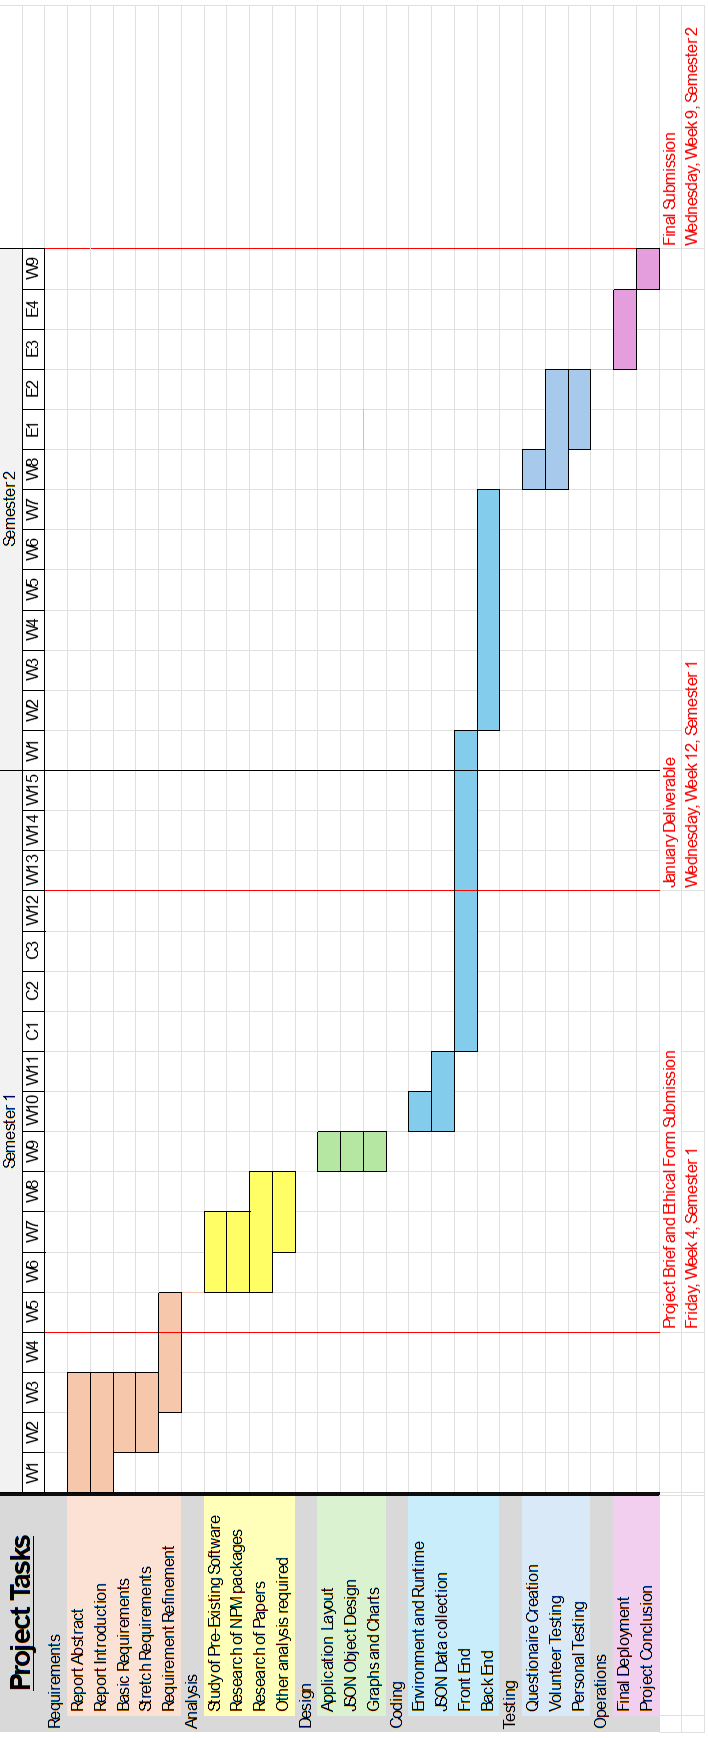
\includegraphics[width=0.4\textwidth, angle=270]{gantt_chart}
        \caption{Gantt Chart}
        \label{fig:gantt_chart}
    \end{figure}
\end{center}
Along with using the Waterfall model, I created a Gantt chart to roughly plan my time for the project. This will help me stay on track and ensure that I am not spending too much time on one section of the project. I will go into further detail about the Gantt chart in the Methodology section of this report.



% This project concerns the visualisation of epidemic data. Specifically the data from the COVID-19 pandemic, but the code will be generic enough to be used for any epidemic data. Visualising the data in a way that is easy to understand is important for understanding the spread of the virus for a wide population.\\
\newpage


\chapter{Problem Domain}
For this project, I will use the MoSCoW structure to define the requirements of the project. This specifies the requirements into layers of priority and sets the scope of my project into perspective.\\
\begin{itemize}
    \item \textbf{\Large{Must Have (Minimum Viable Product)}}
    \begin{itemize}
        \item The dashboard must show a map of the Earth.
        \item The dashboard must visualise the COVID-19 data and show the number of global cases and deaths per week.
        \item The map will render polygon and country data from a GeoJSON file.
        \item The individual countries must be clickable.
        \begin{itemize}
            \item Clicking a country will send the user to a new page.
            \item The new page will show the number of cases and deaths per week.
            \item The new page will show a graph of the number of cases and deaths per week. 
        \end{itemize}
        \item The dashboard must show a timeline of the epidemic.
        \begin{itemize}
            \item The timeline will be a slider.
            \item The user must be able to scrub through the timeline.
            \item The timeline will show the current week.
        \end{itemize}
        \item The user must be able to select data from a file to be displayed.
        \begin{itemize}
            \item The code will accept a clean JSON file.
            \item The JSON file will have the same format as the COVID-19 data.
        \end{itemize}
    \end{itemize}
    \item \textbf{\Large{Should Have}}
    \begin{itemize}
        \item Zooming in on the map.
        \begin{itemize}
            \item This is my most realistic stretch goal. It would require using a library to render the map and allow the user to zoom in and out.
        \end{itemize}
        \item Hotspots on the map.
        \begin{itemize}
            \item This would require analysis of the data to find out where the rate of infection is highest.
        \end{itemize}
    \end{itemize}
    \item \textbf{\Large{Could Have}}
    \begin{itemize}
        \item Analysis of data with other data sources to search for correlations.
        \begin{itemize}
            \item I am currently unsure what data sources I would use for this, but it would be interesting to see if there are any correlations between the spread of the virus and other factors.
        \end{itemize}
    \end{itemize}
    \item \textbf{\Large{Would Have}}
    \begin{itemize}
        \item Predictctive modelling and forecasting.
        \begin{itemize}
            \item This is my most ambitious stretch goal. I would like to be able to predict the spread of the virus using the data I have. This would require a lot of work and research into the field of predictive modelling. This would likely be a separate project in itself.
        \end{itemize}
    \end{itemize}
\end{itemize}
\newpage

\chapter{Methodology}
For this project I will incorperate a Waterfall model into my project since it will ensure my code and report as a whole is developed in a structured and ordered fashion.\\
The steps of Waterfall I will be following are:
\begin{enumerate}
    \item \textbf{\large{Requirements}}
    \begin{itemize}
        \item This section requires producing and refining a set of requirements. I plan on having 2 groups of requirements: Minimum Viable Product requirements and Stretch requirements.
        \item I plan on refining all the requirements in this stage so I can stay on this path plan.
    \end{itemize}
    \item \textbf{\large{Analysis}}
    \begin{itemize}
        \item In this section, I will be doing research into the problems which are discovered by my requirement refinement. I will investigate papers and other relevant published sources.
        \item I also want to investigate node packages to represent my data graphically. (This would continue into the design section)
        \item This section will likely take up a large section of my report, and I may return to this section midway through the project.
    \end{itemize}
    \item \textbf{\large{Design}}
    \begin{itemize}
        \item I would be designing the layout and colour scheme of my application as it would appear in a browser window. It is worth noting that different size screens would render it differently, so I need to take that into account when planning.
        \item I am not using a database for this project, but I will be using JSON and creating a standard design for objects in JSON will be beneficial.
        \item I need to decide what values I use for graphs and what kind of graphs to use.
    \end{itemize}
    \item \textbf{\large{Coding}}
    \begin{itemize}
        \item I will be making a web application with node.js. This will require me to create a valid work environment and get the node runtime working on my local machine. I will likely use Docker for this since it is a very easy to work with tool perfect for this application.
        \item I will mostly be using TypeScript for this project because of type safety and native compatibility with web development. There will also be HTML and CSS for loading the TS canvas and aligning elements.
        \item Node.js also comes with node package manager which will also be useful for loading the custom packages I plan on using in this project.
    \end{itemize}
    \item \textbf{\large{Testing}}
    \begin{itemize}
        \item For testing, I will be using a variety of normal, boundary and erroneous tests to check my software for crashes, unexpected results, and vulnerabilities. Using a type-safe language like TypeScript intends to minimise the chances of these happening.
        \item I also plan on having 3rd-party applicants to test my application. They would have a list of things to do in the application so I can analyse the ease of use.
        \item I would also ask them to fill in a questionnaire.
    \end{itemize}
    \item \textbf{\large{Operations}}
    \begin{itemize}
        \item I want to deploy my application to a server hosted by the university.
        \item Node.js applications are commonly deployed onto servers and having a production repository would be a good standard for myself. Pushing to a server from a local git repository is a highly transferable skill which is widely used. Test
    \end{itemize}
\end{enumerate}
\section{Gantt Chart}
    \begin{center}
        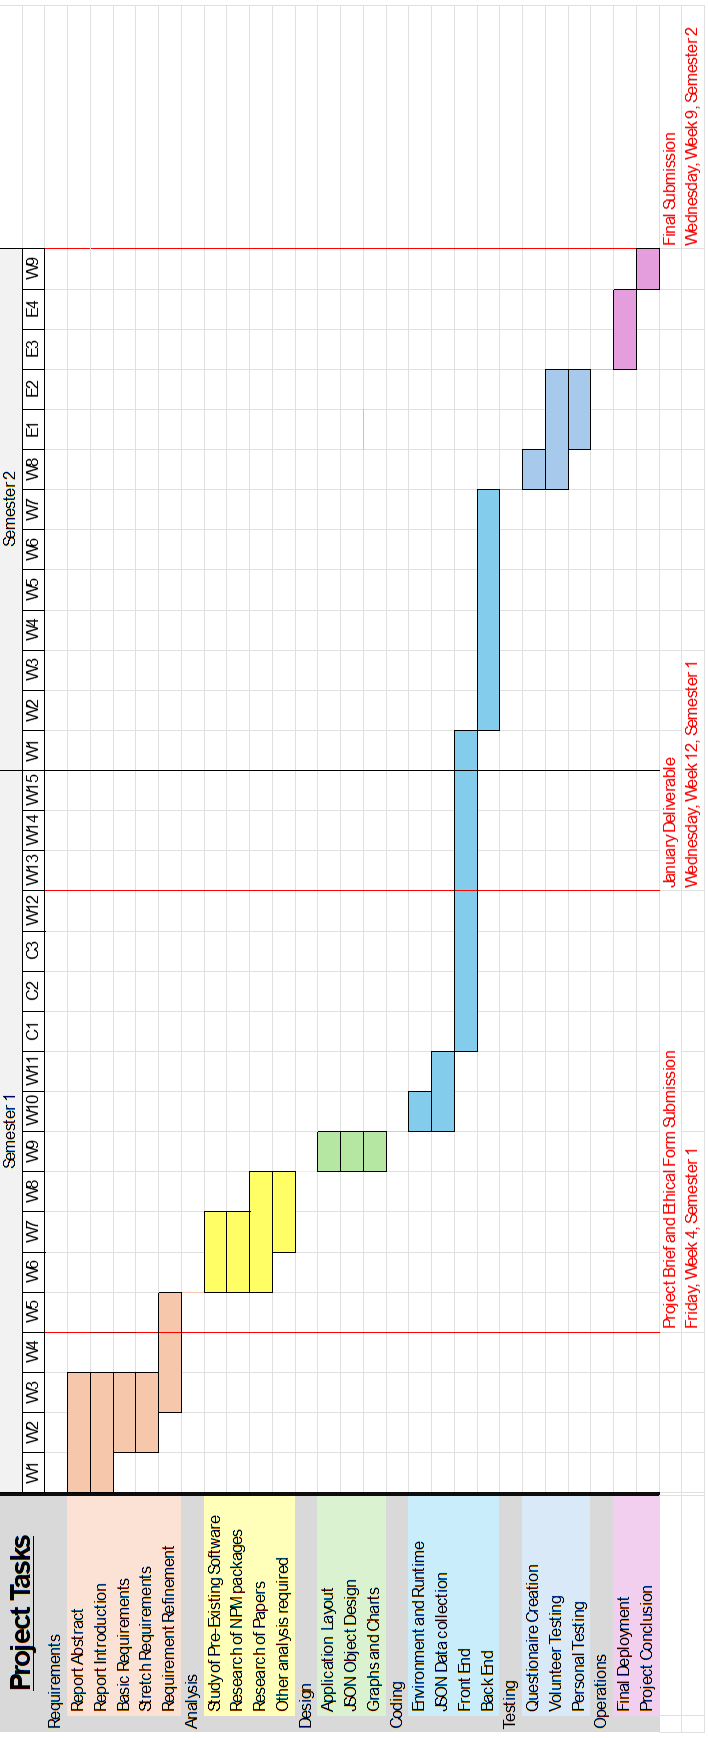
\includegraphics[height=0.95\textheight]{gantt_chart}
    \end{center}

\newpage

\newpage

\chapter{Literature Review}
\section{Existing Solutions}
\subsection{COVID-19 Dashboard}
A common tool for data visualisation is a software called PowerBI, a Microsoft product which allows for the creation of dashboards. 
The dashboard in the figure shows a real-time representation of the COVID-19 pandemic.
\begin{center}
    \begin{figure}[h]
        \centering
        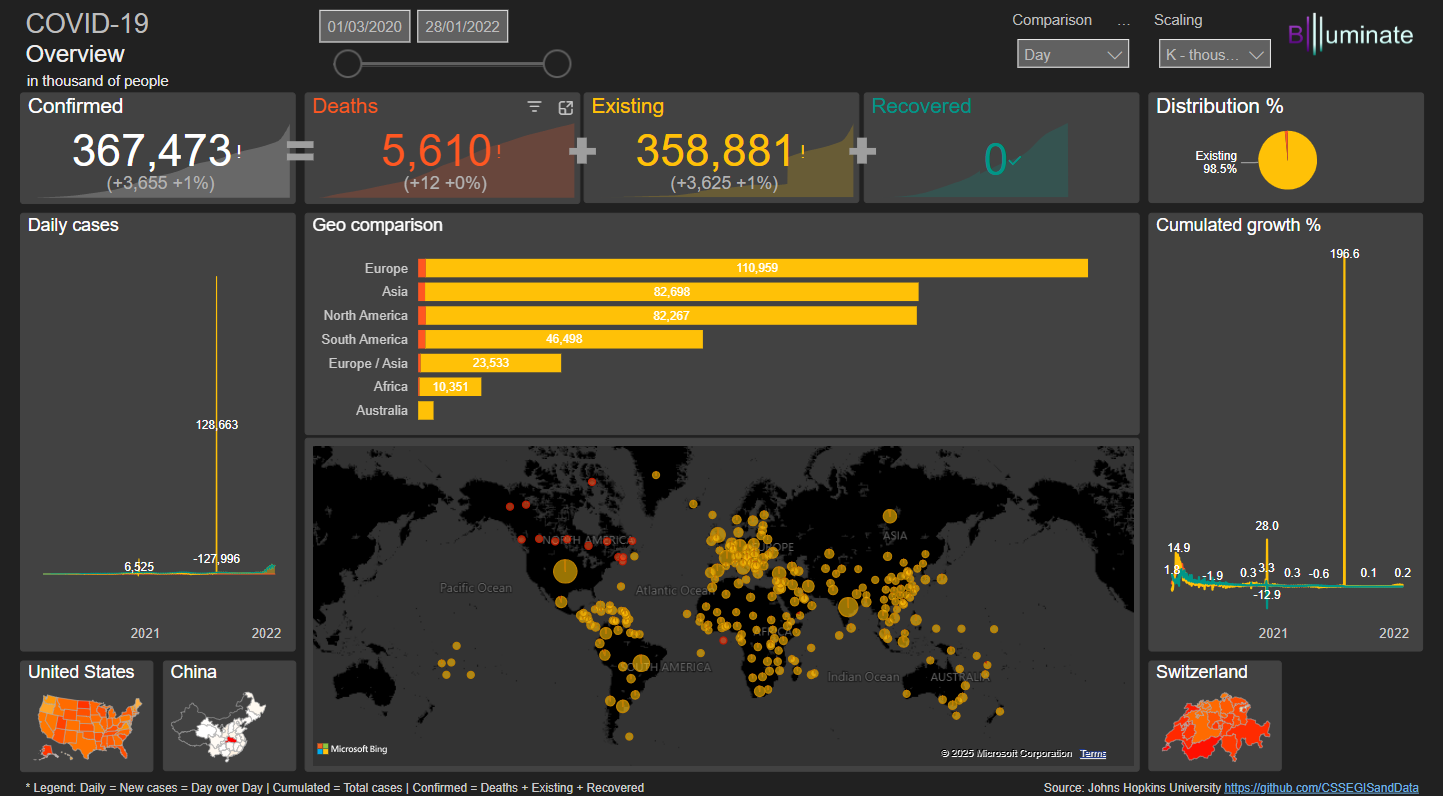
\includegraphics[width=0.95\textwidth]{PowerBI Example.png}
        \caption{COVID-19 Dashboard Example}
        \label{fig:covid19_dashboard}
    \end{figure}
\end{center}

This dashboard has a lot of information on it even at first glance. The map uses bubbles to denote hotspots of activity for the virus. The bubbles are sized by the number of cases in that country. The bubbles can also be clicked for more detailed information on that country. \\
The user is also able to alter the time frame of the data, and the data is updated in real time.\\
There is a lot here which I would like to incorperate into my own project. The map is a good way to visualise the data and the bubbles are a good way to show the number of cases in each country. I also like the big bold text which summarises the data which is easy to read.\\
\newpage
\subsection{Plague Inc.}
Plague Inc. is a game published in 2012 by Ndemic Creations. It gives the user the ability to create and spread a virus across the world. The game was initially released on mobile devices and has since been released on PC and console.\\
Mobiles games require accessible and easy to use interfaces, which is why Plague Inc. is a good example of a visual epidemic simulation. The game is simple to use and has a lot of information on the screen at once.
\begin{center}
    \begin{figure}[h]
        \centering
        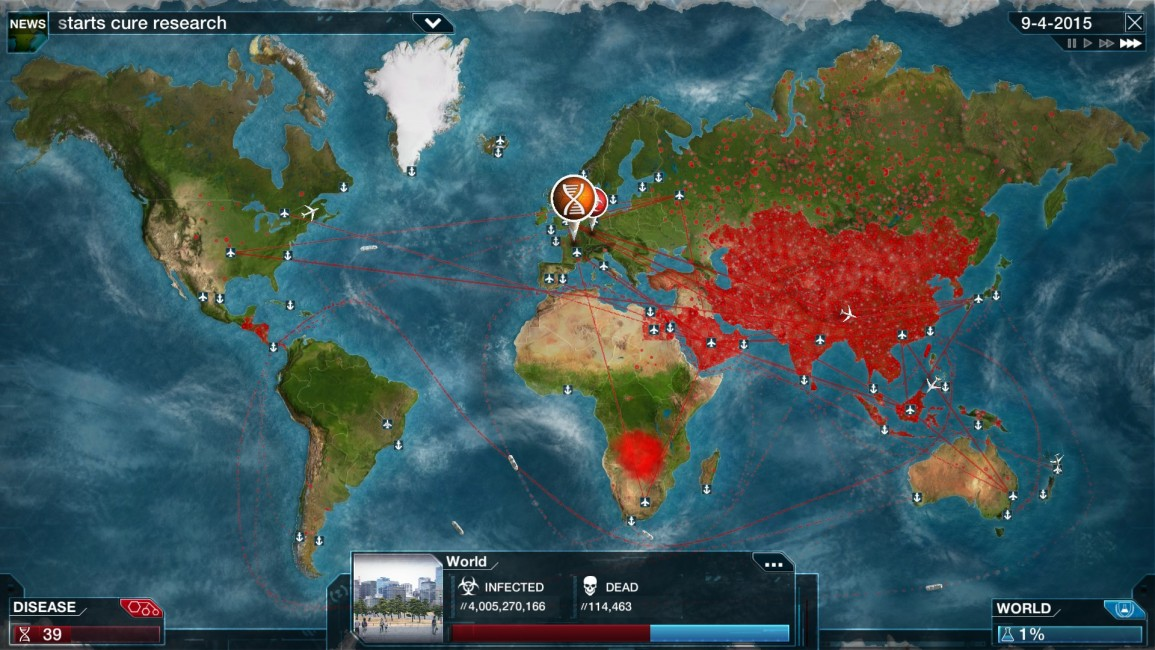
\includegraphics[width=0.95\textwidth]{Plague Inc Example.jpeg}
        \caption{Plague Inc. Dashboard Example}
        \label{fig:plagueinc_dashboard}
    \end{figure}
\end{center}
Despite many systems being dramatised for the sake of gameplay, the game offers many features which could be useful for a real-world epidemic simulation. \\
The game uses a world map which gradually changes colour as the virus spreads, this is from many red dots appearing on the map. The user also has access to individual breakdowns of each country and can see the number of cases and deaths in each country.\\ 
The game also has a transmission system which changes from coutnry to country. 
\\ \\
There is certain information provided in these examples that I will not be able to provide in my project. For example, the COVID-19 dashboard has real-time data, which I will not be able to provide. The Plague Inc. game has a transmission system which changes from country to country, which I will not be able to provide.\\

\newpage
\section{Visualisation}
\subsection{Covid-19 Data Sources}
The data for this project will be sourced from the European Centre for Disease Prevention and Control (ECDC) \cite{ecdc}. The data is historic and only has data from the 1st week of 2020 to the 23rd week of 2022. The data is in a JSON format and includes the number of cases and deaths per week for each country. The format of the data is as follows:

\begin{minipage}{0.45\textwidth}
\begin{lstlisting}[caption={Cases JSON Example}]
{
    "country": "Afghanistan",
    "country_code": "AFG",
    "continent": "Asia",
    "population": 38928341,
    "indicator": "cases",
    "weekly_count": 1368,
    "year_week": "2020-47",
    "rate_14_day": 6.5043,
    "cumulative_count": 44771,
    "source": "Epidemic
    intelligence national data"
}
\end{lstlisting}
\end{minipage}
\hfill
\begin{minipage}{0.45\textwidth}
\begin{lstlisting}[caption={Deaths JSON Example}]
{
    "country": "Afghanistan",
    "country_code": "AFG",
    "continent": "Asia",
    "population": 38928341,
    "indicator": "deaths",
    "weekly_count": 69,
    "year_week": "2020-47",
    "rate_14_day": 3.3395,
    "cumulative_count": 1695,
    "source": "Epidemic
    intelligence national data"
}
\end{lstlisting}
\end{minipage}
This is the format that the ECDC provide, but I will be ammending it slightly to make it easier to work with. I will be combining the cases and deaths into one object and adding a date field. This will make it easier to work with the data in the front end.\\
It also needs to correspond with the GeoJSON data I will be using to render the map. \\
It is worth noting that I don't want this code to be limited to just COVID-19 data. I want to be able to use this code for any epidemic data. This is why I am making the data more generic and easier to work with.\\
\newpage
\section{Compartmental Models}
\subsection{SIR Model}
Compartmental models are a type of mathematical model used to represent the different populations in a system. The most common compartmental system in epidemiology is the SIR model \cite{beckley2013modeling}.\\
The SIR model is a simple model which divides the population into three compartments: Susceptible, Infected and Recovered. The model is represented by the following differential equations:
\begin{align}
\frac{dS}{dt} &= -\alpha SI \label{sir_model_dS} \\
\frac{dI}{dt} &= \alpha SI - \beta I \label{sir_model_dI} \\
\frac{dR}{dt} &= \beta I \label{sir_model_dR}
\end{align}
Where:
\begin{itemize}
    \item S is the number of susceptible individuals.
    \item I is the number of infected individuals.
    \item R is the number of recovered individuals.
    \item $\alpha$ is the rate of infection.
    \item $\beta$ is the rate of recovery.
\end{itemize}
To explain this model, it's important to understand proportional reasoning. In the first equation, \ref{sir_model_dS}, the rate of change of the susceptible population is proportional to the complement of the product of the susceptible and infected populations.\\
A way to think of why that is true is because the more infected people there are, the more likely it is for a susceptible person to become infected.\\
This model is a good starting point for undestanding the spread of a virus, but it has some limitations. In this model, once you have recovered, you are no longer able to be infected. Another issue is that the model assumes the disease is non-fatal.

\subsection{Solution to the SIR Model}
The SIR model can be solved using numerical methods. The most common method is the Euler method. The Euler method is a simple method for solving ordinary differential equations. It is not the most accurate method, but it is easy to implement. The Euler method is represented by the following equations:
\begin{align}
S_{n+1} &= S_n - \alpha S_n I_n \Delta t \label{sir_euler_S} \\
I_{n+1} &= I_n + \alpha S_n I_n \Delta t - \beta I_n \Delta t \label{sir_euler_I} \\
R_{n+1} &= R_n + \beta I_n \Delta t \label{sir_euler_R}
\end{align}
Where:
\begin{itemize}
    \item $S_n$ is the number of susceptible individuals at time $n$.
    \item $I_n$ is the number of infected individuals at time $n$.
    \item $R_n$ is the number of recovered individuals at time $n$.
    \item $\Delta t$ is the time step.
\end{itemize}
If we look at the phase space of the SIR model, we can see that the model has a fixed point at the origin. This means that the model will always return to the origin. This is not the case in real life, as the disease will eventually die out. This is because the model does not take into account the finite population size.\\

\subsection{Improvements to the SIR Model}
The SIR model can be improved by adding more compartments to the model. However, this makes the model more complex and harder to solve.
\subsubsection{SEIR Model}
This model adds an exposed compartment to the SIR model. For individuals who have been infected but are not yet infectious. The model is represented by the following differential equations:
\begin{align}
\frac{dS}{dt} &= \mu N - \mu S - \frac{\beta IS}{N} \label{seir_model_dS} \\
\frac{dE}{dt} &= \frac{\beta IS}{N} - (\mu + a)E \label{seir_model_dE} \\
\frac{dI}{dt} &= aE - (\mu + \gamma)I \label{seir_model_dI} \\
\frac{dR}{dt} &= \gamma I - \mu R \label{seir_model_dR}
\end{align}
The SEIR model is better for simulations than the SIR model since it takes into account the incubation period of the disease. This is important as it is possible for a person to be infected but not yet infectious.\\
It is beyond the scope of this project to go into detail about the SEIR model, but it is worth noting that the model is more complex and requires more data to solve. The model is also more accurate than the SIR model.

\chapter{Design Review}
\section{Wireframing}
I need to work within the constraints of node.js and D3.js for my designs. Below is a wireframe of the dashboard I plan on creating.\\
\begin{center}
    \begin{figure}[h]
        \centering
        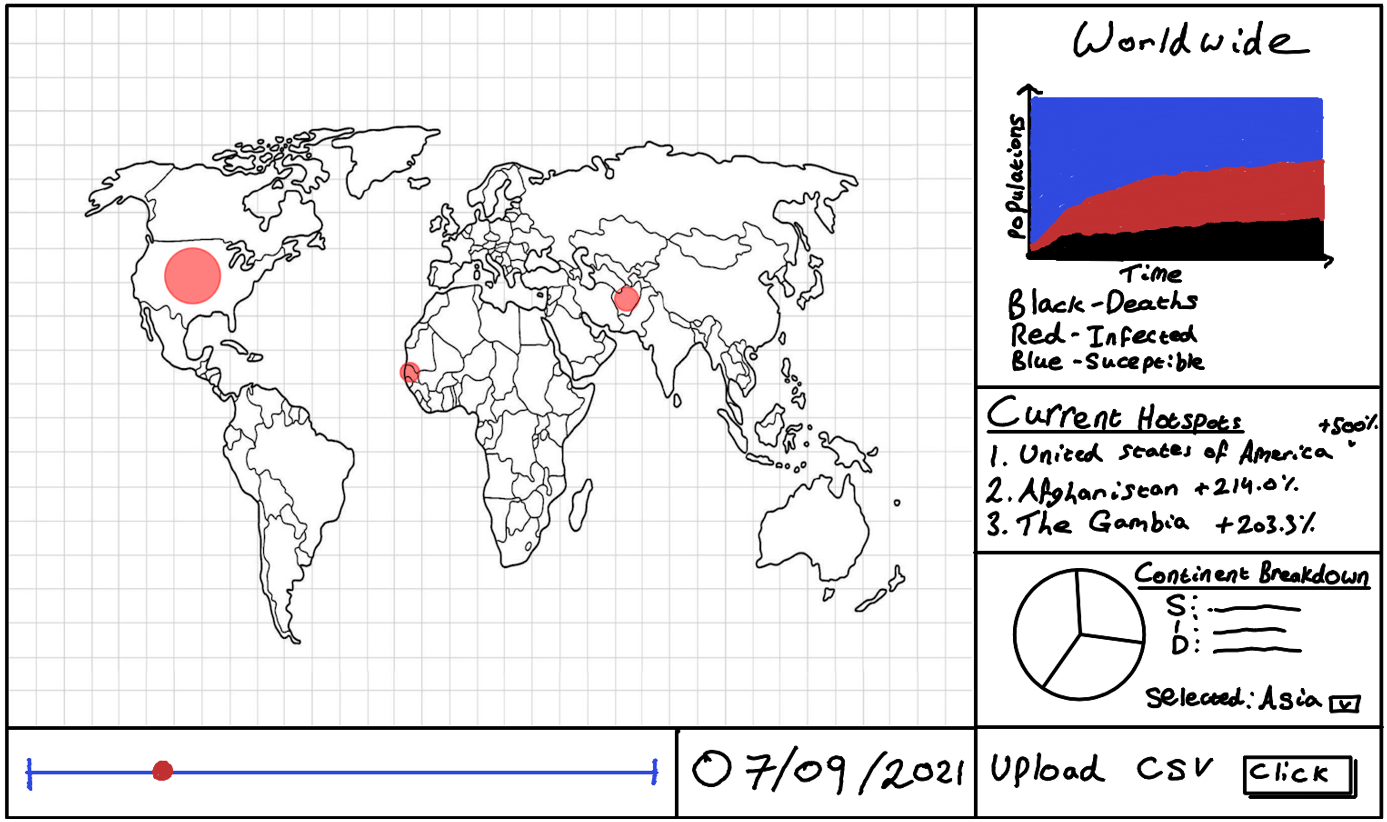
\includegraphics[width=0.95\textwidth]{Images/Home_Wireframe.png}
        \caption{Wireframe of Dashboard}
        \label{fig:wireframe_world}
    \end{figure}
\end{center}
Specific features of the dashboard include:
\begin{itemize}
    \item A map of the Earth.
    \item An interactive timeline of the epidemic.
    \item A area chart showing the number of cases, deaths and population susceptible.
    \item Listed hotspots and the percentage change within the countries.
    \item Hotspots on the map.
    \item A pie chart for susceptible, infected and dead populations within continents.
    \item A button to load different data files.
    \item The current date in the data.
\end{itemize}
When clicking on a country, the canvas will zoom onto the country, giving more specific information on how the pandemic is affecting that country. A button will also be available to return to the world map.
\begin{center}
    \begin{figure}[h]
        \centering
        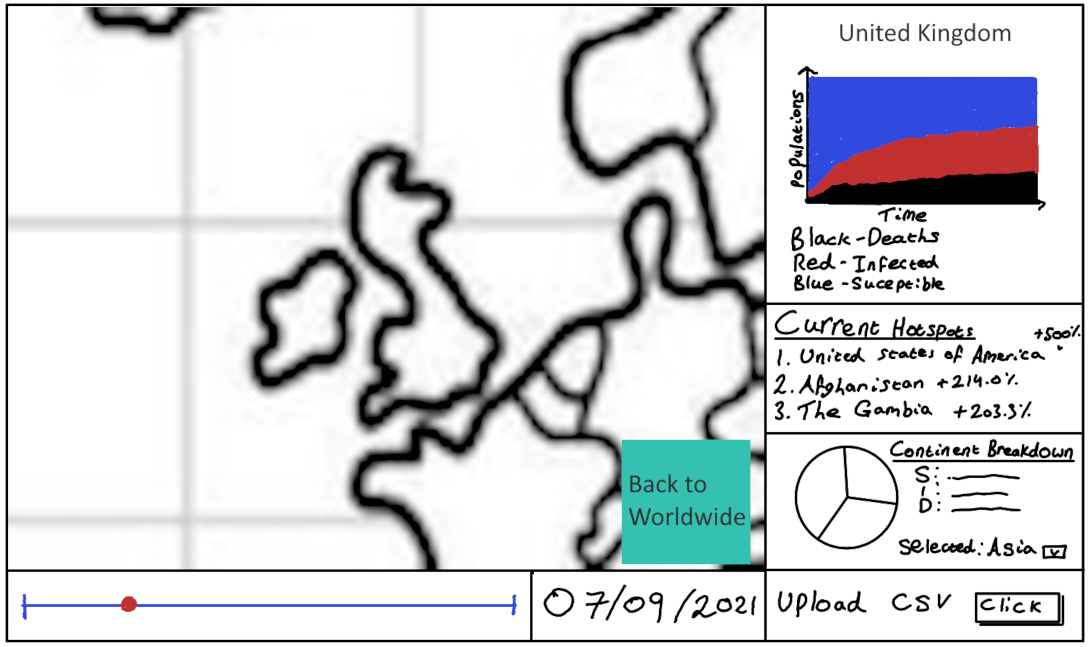
\includegraphics[width=0.95\textwidth]{Images/Country_Wireframe.png}
        \caption{Wireframe of Country Page}
        \label{fig:wireframe_country}
    \end{figure}
\end{center}
A perk of using SVG to render the map is that when zooming, no resolution is lost. This is because SVG is a vector format, meaning that the image is made up of lines and shapes rather than pixels. This means that the image can be scaled up and down without losing quality.
\section{D3.js}
D3.js is a JavaScript library for producing dynamic, interactive data visualisations in web browsers. It makes use of the widely supported SVG format to render graphics. D3.js is a powerful tool for creating visualisations and is widely used in industry.

D3.js is a good choice for this project as it natively supports GeoJSON data which is the format I will be using for the map. \cite{geojsonvectormaps}

This is exclusively used on a web browser, so I will be using node.js to serve the data to the front end.
\newpage
The GeoJSON data has much more information than the COVID-19 data. It includes geometry of the country, information regarding the countries economy, sovereign status, GDP, all in multiple languages. I will be cleaning the data to only include relevant information for this project: country name in English, country code (to link the data with the Covid-19 JSON file) and geometry information. 

\section{Statistical Analysis}
Statistical analysis is a key part of this project. I will be using statistical analysis to find correlations between the data and other factors. I will be comparing the cumulative cases and deaths of two countries to see if there are any correlations between the two.\\

I also want to make a statistic comparing the number of cases to the gdp per capita of the country to see if there is an inverse correlation between the two. This would be interesting to see richer countries were able to contain the virus better than poorer countries.
\begin{align}
\text{Infections} &\propto \frac{1}{\text{GDP Per Capita}}
\end{align}

If this is the case, I would like to calculate the constant of proportionality. This would be a good indicator of how much money a country needs to spend to contain the virus. \\

I would also like to compare number of cases to other statistics I have available to me in my GeoJSON file. This includes:
\begin{itemize}
    \item Population
    \item Sovereign status
    \item Type of economy
    \item etc
\end{itemize}

\newpage
\chapter{Technical Solution}
\section{Cleaning the Data}
Before I start working on the front end, I need to clean the data. The data from the ECDC is in a JSON format, but it is not in a format that is easy to work with. I need to combine the cases and deaths into one object and add a date field. This will make it easier to work with the data in the front end.

I will be using Python to clean the data, since doing this is a one-time task and Python is a good language for data manipulation. I will be using the Pandas library to read the JSON file and manipulate the data. I will then write the cleaned data to a new JSON file.

I restrucutred the data to look like this:
\begin{center}
    \begin{lstlisting}
    {
        "Afghanistan": {
            "properties": {
                "country": "Afghanistan",
                "country_code": "AFG",
                "continent": "Asia",
                "population": 38928341,
                "source": "Epidemic intelligence national data"
            },
            "data": {
                "2020-01": {
                    "cases": 0,
                    "deaths": 0,
                    "cumulative_cases": 0,
                    "cumulative_deaths": 0
                },
                [...]
            }
        },
        [...]
    }
    \end{lstlisting}
\end{center}
The python code I used can be found in the appendix.

\section{Country Selection}
For this project, I need to decide on what list of countries to use. The GeoJSON file I will be using has a selection of countries, but a definitive list of countries doesn't exist.

There are multiple countries that are in dispute due to political or territorial reasons. For example, Taiwan is not recognised as a country by the United Nations due to China needing to agree, but it is a country in its own right. I will be including Taiwan in my list of countries.

Another consideration are countries which aren't included in the $\mathbf{ISO}$ $\mathbf{3166-1}$ $\mathbf{Alpha-3}$ country code set which is what both the ECDC and GeoJSON file use. An example is Somaliland which is a self-declared state but is not recognised by the United Nations or the ISO-3166-1 country code, but the dataset does contain data so we will extend the country code set to include this.

There are multiple more examples like this, here is a list of countries I will be including in my dataset:
\newpage
\begin{center}
    \begin{minipage}{0.46\textwidth}
        \begin{tabular}{|p{10.5em}|p{6em}|}
            \hline
            Country or Area Name & ISO Code\\
            \hline
            Afghanistan & AFG\\
            Africa (total) & N/A\\
            Albania & ALB\\
            Algeria & DZA\\
            America (total) & N/A\\
            American Samoa & ASM\\
            Andorra & AND\\
            Angola & AGO\\
            Anguilla & AIA\\
            Antigua And Barbuda & ATG\\
            Argentina & ARG\\
            Armenia & ARM\\
            Aruba & ABW\\
            Asia (total) & N/A\\
            Australia & AUS\\
            Austria & AUT\\
            Azerbaijan & AZE\\
            Bahamas & BHS\\
            Bahrain & BHR\\
            Bangladesh & BGD\\
            Barbados & BRB\\
            Belarus & BLR\\
            Belgium & BEL\\
            Belize & BLZ\\
            Benin & BEN\\
            Bermuda & BMU\\
            Bhutan & BTN\\
            Bolivia & BOL\\
            Bonaire, Saint Eustatius And Saba & BES\\
            Bosnia And Herzegovina & BIH\\
            Botswana & BWA\\
            Brazil & BRA\\
            British Virgin Islands & VGB\\
            Brunei Darussalam & BRN\\
            Bulgaria & BGR\\
            Burkina Faso & BFA\\
            Burundi & BDI\\
            Cambodia & KHM\\
            Cameroon & CMR\\
            Canada & CAN\\
            Cape Verde & CPV\\
            Cayman Islands & CYM\\
            Central African Republic & CAF\\
            Chad & TCD\\
            \hline
        \end{tabular}
    \end{minipage}
    \hfill
    \begin{minipage}{0.46\textwidth}
        \begin{tabular}{|p{10.5em}|p{6em}|}
            \hline
            Country or Area Name & ISO Code\\
            \hline
            Chile & CHL\\
            China & CHN\\
            Colombia & COL\\
            Comoros & COM\\
            Congo & COG\\
            Cook Islands & COK\\
            Costa Rica & CRI\\
            Cote Divoire & CIV\\
            Croatia & HRV\\
            Cuba & CUB\\
            Curaçao & CUW\\
            Czechia & CZE\\
            Democratic Republic Of The Congo & COD\\
            Denmark & DNK\\
            Djibouti & DJI\\
            Dominica & DMA\\
            Dominican Republic & DOM\\
            Ecuador & ECU\\
            Egypt & EGY\\
            El Salvador & SLV\\
            Equatorial Guinea & GNQ\\
            Eritrea & ERI\\
            Estonia & EST\\
            Eswatini & SWZ\\
            Ethiopia & ETH\\
            EU/EEA (total) & N/A\\
            Europe (total) & N/A\\
            Falkland Islands (Malvinas) & FLK\\
            Faroe Islands & FRO\\
            Fiji & FJI\\
            Finland & FIN\\
            France & FRA\\
            French Polynesia & PYF\\
            Gabon & GAB\\
            Gambia & GMB\\
            Georgia & GEO\\
            Germany & DEU\\
            Ghana & GHA\\
            Gibraltar & GIB\\
            Greece & GRC\\
            Greenland & GRL\\
            Grenada & GRD\\
            Guam & GUM\\
            Guatemala & GTM\\
            Guernsey & GGY\\
            \hline
        \end{tabular}
    \end{minipage}

    \newpage
    \begin{minipage}{0.46\textwidth}
        \begin{tabular}{|p{10.5em}|p{6em}|}
            \hline
            Country or Area Name & ISO Code\\
            \hline
            Guinea & GIN\\
            Guinea Bissau & GNB\\
            Guyana & GUY\\
            Haiti & HTI\\
            Holy See & VAT\\
            Honduras & HND\\
            Hungary & HUN\\
            Iceland & ISL\\
            India & IND\\
            Indonesia & IDN\\
            Iran & IRN\\
            Iraq & IRQ\\
            Ireland & IRL\\
            Isle Of Man & IMN\\
            Israel & ISR\\
            Italy & ITA\\
            Jamaica & JAM\\
            Japan & JPN\\
            Jersey & JEY\\
            Jordan & JOR\\
            Kazakhstan & KAZ\\
            Kenya & KEN\\
            Kiribati & KIR\\
            Kosovo & XKX\\
            Kuwait & KWT\\
            Kyrgyzstan & KGZ\\
            Laos & LAO\\
            Latvia & LVA\\
            Lebanon & LBN\\
            Lesotho & LSO\\
            Liberia & LBR\\
            Libya & LBY\\
            Liechtenstein & LIE\\
            Lithuania & LTU\\
            Luxembourg & LUX\\
            Madagascar & MDG\\
            Malawi & MWI\\
            Malaysia & MYS\\
            Maldives & MDV\\
            Mali & MLI\\
            Malta & MLT\\
            Marshall Islands & MHL\\
            Mauritania & MRT\\
            Mauritius & MUS\\
            Mexico & MEX\\
            Micronesia (Federated States Of) & FSM\\
            \hline
        \end{tabular}
    \end{minipage}
    \hfill
    \begin{minipage}{0.46\textwidth}
        \begin{tabular}{|p{10.5em}|p{6em}|}
            \hline
            Country or Area Name & ISO Code\\
            \hline
            Moldova & MDA\\
            Monaco & MCO\\
            Mongolia & MNG\\
            Montenegro & MNE\\
            Montserrat & MSR\\
            Morocco & MAR\\
            Mozambique & MOZ\\
            Myanmar & MMR\\
            Namibia & NAM\\
            Nauru & NRU\\
            Nepal & NPL\\
            Netherlands & NLD\\
            New Caledonia & NCL\\
            New Zealand & NZL\\
            Nicaragua & NIC\\
            Niger & NER\\
            Nigeria & NGA\\
            North Macedonia & MKD\\
            Northern Mariana Islands & MNP\\
            Norway & NOR\\
            Oceania (total) & N/A\\
            Oman & OMN\\
            Pakistan & PAK\\
            Palau & PLW\\
            Palestine & PSE\\
            Panama & PAN\\
            Papua New Guinea & PNG\\
            Paraguay & PRY\\
            Peru & PER\\
            Philippines & PHL\\
            Poland & POL\\
            Portugal & PRT\\
            Puerto Rico & PRI\\
            Qatar & QAT\\
            Romania & ROU\\
            Republic of Türkiye & TUR\\
            Russia & RUS\\
            Rwanda & RWA\\
            Saint Kitts And Nevis & KNA\\
            Saint Lucia & LCA\\
            Saint Vincent And The Grenadines & VCT\\
            Samoa & WSM\\
            San Marino & SMR\\
            Sao Tome And Principe & STP\\
            Saudi Arabia & SAU\\
            \hline
        \end{tabular}
    \end{minipage}

    \newpage
    \begin{minipage}{0.46\textwidth}
        \begin{tabular}{|p{10.5em}|p{6em}|}
            \hline
            Country or Area Name & ISO Code\\
            \hline
            Senegal & SEN\\
            Serbia & SRB\\
            Seychelles & SYC\\
            Sierra Leone & SLE\\
            Singapore & SGP\\
            Sint Maarten & SXM\\
            Slovakia & SVK\\
            Slovenia & SVN\\
            Solomon Islands & SLB\\
            Somalia & SOM\\
            South Africa & ZAF\\
            South Korea & KOR\\
            South Sudan & SSD\\
            Spain & ESP\\
            Sri Lanka & LKA\\
            Sudan & SDN\\
            Suriname & SUR\\
            Sweden & SWE\\
            Switzerland & CHE\\
            Syria & SYR\\
            Taiwan & TWN\\
            Tajikistan & TJK\\
            Thailand & THA\\
            Timor Leste & TLS\\
            Togo & TGO\\
            Tonga & TON\\
            Trinidad And Tobago & TTO\\
            Tunisia & TUN\\
            Turks And Caicos Islands & TCA\\
            Tuvalu & TUV\\
            Uganda & UGA\\
            Ukraine & UKR\\
            United Arab Emirates & ARE\\
            United Kingdom & GBR\\
            United Republic Of Tanzania & TZA\\
            United States Of America & USA\\
            United States Virgin Islands & VIR\\
            Uruguay & URY\\
            Uzbekistan & UZB\\
            \hline
        \end{tabular}
    \end{minipage}
    \hfill
    \begin{minipage}{0.46\textwidth}
        \begin{tabular}{|p{10.5em}|p{6em}|}
            \hline
            Country or Area Name & ISO Code\\
            \hline
            Vanuatu & VUT\\
            Venezuela & VEN\\
            Vietnam & VNM\\
            Wallis And Futuna & WLF\\
            Western Sahara & ESH\\
            Yemen & YEM\\
            Zambia & ZMB\\
            Zimbabwe & ZWE\\
            Cyprus & CYP\\
            \hline
        \end{tabular}
    \end{minipage}
\end{center}

\newpage

Initially, I wanted to use UNIX timestamps to store the date, but I have since changed my mind. This is because of of how the HTML slider tag works. The slider expects consistent step values, and UNIX timestamps are not consistent due to daylight savings time.

To combat this, I am storing data in the string form of "YYYY-ww" where YYYY is the year and ww is the week number. This is a consistent format and will work with the HTML slider tag. I will have a function to convert the string to a date object when I need to use it.

\section{Frontend}

\subsection{World Map}
The world map in this project was a success in planning. I used the D3.js library to render the map and it worked well. The map is interactive and allows the user to zoom in on countries.

I was able to take advantage of features in D3.js like transisition and zoom for a smoother feel to the map. The chloropleth map is a good way to represent the data and allows the user to see the hotspots of the virus.

I used the GeoJSON polygon data to render the map. This had many beneficial side effects, like: Choice of projection, the multipolygon feature of GeoJSON, rendering the data in SVG format, and the ability to use D3.js features like transitions and zoom.

\subsection{Info Panel}
Originally, I planned to use a stacked area chart for this project, but I have since changed my mind. The reason is that the stacked area chart is not a good way to represent the data. The populations of the susceptible and the cases/deaths are very disproportionate so a linear scale would not work. Instead, I will be using a logarithmic scale for the y-axis. This will allow me to show the data in a more meaningful way.

The area chart will be a simple line chart with the x-axis being the date and the y-axis being the size of the populations. The chart will have a legend to show what each line represents. The chart will also have a title and axis labels.

\section{Backend}
For the data in my application, I am using the file "interface.js" to load the data from the JSON file. This file is an async module which exports a function to load the data. The function can fetch all data or data specfied in the parameters. The function will return a promise which resolves to the data. This is a simple way to load data from a file and is a common pattern in JavaScript.

This is my first time ever dealing with async functions and promises.

\chapter{Results and Analysis}
\newpage

\chapter{Conclusion}

\newpage

\bibliographystyle{plain} % We choose the "plain" reference style
\bibliography{refs} % Entries are in the refs.bib file


\newpage

\chapter{Appendix}
\section{restrucure-json.py}
\begin{lstlisting}[language=Python]
import json
from collections import defaultdict

# Load JSON data from file
with open("data.json", "r", encoding="utf-8") as infile:
    json_data = json.load(infile)

# Transform data
result = defaultdict(lambda: {"properties": {},
                              "data": defaultdict(lambda:
                                      {"cases": 0,
                                       "deaths": 0,
                                       "cumulative_cases": 0,
                                       "cumulative_deaths": 0})})

for entry in json_data:
    try:
        country = entry["country"]
        
        # Populate properties
        if not result[country]["properties"]:
            result[country]["properties"] = {
                "country": entry.get("country", "Unknown"),
                "country_code": entry.get("country_code", "N/A"),
                "continent": entry.get("continent", "Unknown"),
                "population": entry.get("population", 0),
                "source": entry.get("source", "Unknown")
            }

        # Organize data by year_week
        year_week = entry.get("year_week", "Unknown")
        weekly_count = entry.get("weekly_count", 0)
        cumulative_count = entry.get("cumulative_count", 0)
        indicator = entry.get("indicator", "").lower()

        if indicator == "cases":
            result[country]["data"][year_week]["cases"]
                        = weekly_count
            result[country]["data"][year_week]["cumulative_cases"]
                        = cumulative_count
        elif indicator == "deaths":
            result[country]["data"][year_week]["deaths"]
                        = weekly_count
            result[country]["data"][year_week]["cumulative_deaths"]
                        = cumulative_count
    except KeyError as e:
        print(f"Missing key {e} in entry: {entry}")

# Convert defaultdict to normal dict
final_result = {country: {"properties": data["properties"],
        "data": dict(data["data"])} for country, data in result.items()}

# Write output to a new JSON file
with open("restructured_data.json", "w", encoding="utf-8") as outfile:
    json.dump(final_result, outfile, indent=4)

print("Data successfully transformed and saved to 'new_data.json'")
\end{lstlisting}


\newpage




\end{document}